\documentclass[twoside]{article}

\usepackage{aistats2022}
% If your paper is accepted, change the options for the package
% aistats2022 as follows:
%
%\usepackage[accepted]{aistats2022}
%
% This option will print headings for the title of your paper and
% headings for the authors names, plus a copyright note at the end of
% the first column of the first page.

% If you set papersize explicitly, activate the following three lines:
%\special{papersize = 8.5in, 11in}
%\setlength{\pdfpageheight}{11in}
%\setlength{\pdfpagewidth}{8.5in}

% If you use natbib package, activate the following three lines:
\usepackage[round]{natbib}
\renewcommand{\bibname}{References}
\renewcommand{\bibsection}{\subsubsection*{\bibname}}

% If you use BibTeX in apalike style, activate the following line:
%\bibliographystyle{apalike}
\usepackage[utf8]{inputenc} % allow utf-8 input
\usepackage[T1]{fontenc}    % use 8-bit T1 fonts
\usepackage{hyperref}       % hyperlinks
\usepackage{url}            % simple URL typesetting
\usepackage{booktabs}       % professional-quality tables
\usepackage{amsfonts}       % blackboard math symbols
\usepackage{nicefrac}       % compact symbols for 1/2, etc.
\usepackage{microtype}      % microtypography
\usepackage{xcolor}         % colors
\usepackage{makecell}

% ==============================
% My packages
\usepackage{amsmath}
\usepackage{svg}
\usepackage{pdfpages}
\usepackage{wrapfig}
\usepackage{longtable}
\usepackage{lipsum}
\usepackage[ruled]{algorithm2e}
\usepackage{graphicx,multirow}
\usepackage{xfrac}
\usepackage{subcaption}
\usepackage{csvsimple}
\usepackage{lscape}
\usepackage[normalem]{ulem}
\input{math}



% Unnumber algoright
% \makeatletter
% \newcommand{\RemoveAlgoNumber}{\renewcommand{\fnum@algocf}{\AlCapSty{\AlCapFnt\algorithmcfname}}}
% \newcommand{\RevertAlgoNumber}{\algocf@resetfnum}
% \makeatother

% Colours
\definecolor{navyBlue}{HTML}{030F4F}
\definecolor{primaryRed}{HTML}{990000}
\definecolor{editGreen}{HTML}{40916c}
\definecolor{gray}{HTML}{aaaaaa}

% My inputs
%\input{setup/math}
\bibliographystyle{unsrtnat}

\begin{document}

\twocolumn[
\aistatstitle{Robust uncertainty estimates with out-of-distribution pseudo-inputs training}

\aistatsauthor{ Pierre Segonne \And Yevgen Zainchkovskyy \And  Søren Hauberg}

\aistatsaddress{ Institution 1 \And  Institution 2 \And Institution 3 } ]

\begin{abstract}
  Probabilistic models often use neural networks to control their predictive uncertainty.
  However, when making \textit{out-of-distribution (OOD)} predictions, the often-uncontrollable 
  extrapolation properties of neural networks yield poor uncertainty predictions. Such models then don't \textit{know what they don't know}, which directly limits their robustness w.r.t unexpected inputs.
  To counter this, we propose to explicitly train the uncertainty predictor where we are not given data
  to make it reliable. As one cannot train without data, we provide mechanisms for generating
  \emph{pseudo-inputs} in informative low-density regions of the input space, and show how to leverage these in a practical
  Bayesian framework that casts a prior distribution over the model uncertainty. With a holistic evaluation, we demonstrate that this yields robust and interpretable predictions of uncertainty while retaining
  state-of-the-art performance on diverse tasks such as regression and generative modelling.\looseness=-1
\end{abstract}

% ==========================
% \input{sections/introduction}
% \input{sections/method}
% \section{Experiments}
% \input{sections/regression}
% \input{sections/generative_modelling}
% \input{sections/conclusion}
% ==========================

% ==========================
% DO NOT INCLUDE AT SUBMISSION TIME
% \textbf{\large Acknowledgements.} ...
\section{Lipsum}
% \resizebox{\columnwidth}{!}{%
% \begin{tabular}{lllll}
% \toprule
%       & & FashionMNIST & SVHN & CIFAR \\
% \midrule
% \multirow{2}{*}{$\log p(\rx)$} & VAE & $2215.54\pm68.81$ & $\mathbf{4304.90\pm58.45}$  & $\mathbf{2930.64\pm14.82}$    \\
%   & d-V3AE & $\mathbf{2349.71\pm11.80}$ & $4133.41\pm 64.28$ & $2668.85\pm13.23$\\
% \multirow{2}{*}{$\text{RMSE}(\rx,\tilde{\rx})$} & VAE & $0.171\pm0.003$ & $0.097\pm7\text{e-}4$  & $0.154\pm5\text{e-}4$    \\
%   & d-V3AE & $\mathbf{0.158\pm0.003}$ & $\mathbf{0.087\pm0.002}$ & $\mathbf{0.129\pm7\text{e-}4}$\\
% \bottomrule
% \end{tabular}
% }

\resizebox{\columnwidth}{!}{%
\setcellgapes{3pt}
\makegapedcells
\begin{tabular}{@{\hskip0pt}llr@{$\pm$}lr@{$\pm$}lr@{$\pm$}lr@{$\pm$}lr@{$\pm$}lr@{$\pm$}l}
\toprule
      & & \multicolumn{2}{l}{FashionMNIST} & \multicolumn{2}{l}{SVHN} & \multicolumn{2}{l}{CIFAR} \\
\midrule
\multirow{2}{*}{\rotatebox[origin=c]{0}{$\log p(\rx)$}} & VAE & $2215.54$ & $68.81$ & $\mathbf{4304.90}$ & $\mathbf{58.45}$ & $\mathbf{2930.64}$ & $\mathbf{14.82}$    \\
  & d-V3AE & $\mathbf{2349.71}$ & $\mathbf{11.80}$ & $4133.41$ & $64.28$ & $2668.85$ & $13.23$\\
\multirow{2}{*}{\rotatebox[origin=c]{0}{$\text{RMSE}(\rx,\tilde{\rx})$}} & VAE & $0.171$ & $0.003$ & $0.097$ & $7\text{e-}4$ & $0.154$ & $5\text{e-}4$    \\
  & d-V3AE & $\mathbf{0.158}$ & $\mathbf{0.003}$ & $\mathbf{0.087}$ & $\mathbf{0.002}$ & $\mathbf{0.129}$ & $\mathbf{7\text{e-}4}$\\
\bottomrule
\end{tabular}
}


\begin{table*}[h]
\caption{UCI benchmarks over 5 trials. Each cell counts the number of datasets for which each method demonstrated the best average. Grey shows statistical draws and "n/a" metrics impossible to evaluate for a method.  Best per metric is highlighted in bold.\looseness=-1}
\label{tab:uci_no_shifts}
\input{../output/0-table-summary-no-shifts.tex}
\end{table*}

\begin{table*}[h]
\caption{UCI benchmarks over 5 trials. Each cell counts the number of datasets for which each method demonstrated the best average. Grey shows statistical draws and "n/a" metrics impossible to evaluate for a method.  Best per metric is highlighted in bold.\looseness=-1}
\label{tab:uci_only_shifts}
\input{../output/0-table-summary-only-shifts.tex}
\end{table*}

% \begin{figure*}[t!]
    \begin{minipage}[t]{.33\textwidth}
    %   \centering
      \includegraphics[width=\textwidth]{assets/vae_variance_plots.pdf} % \includegraphics[height=5cm]{assets/vae_variance_plots.pdf}
      \vspace{-2.5mm}
      \captionof{figure}{Decoder's aggregated variance (left) and generated samples (right) from the latent space. Coloured points correspond to latent representations of test data, with per-class colours.}
      \label{fig:vae_variance_plots}
    \end{minipage}%
    \hspace{.02\textwidth}
    \begin{minipage}[t]{.39\textwidth}
        \vspace{-5cm}
    %   \centering
      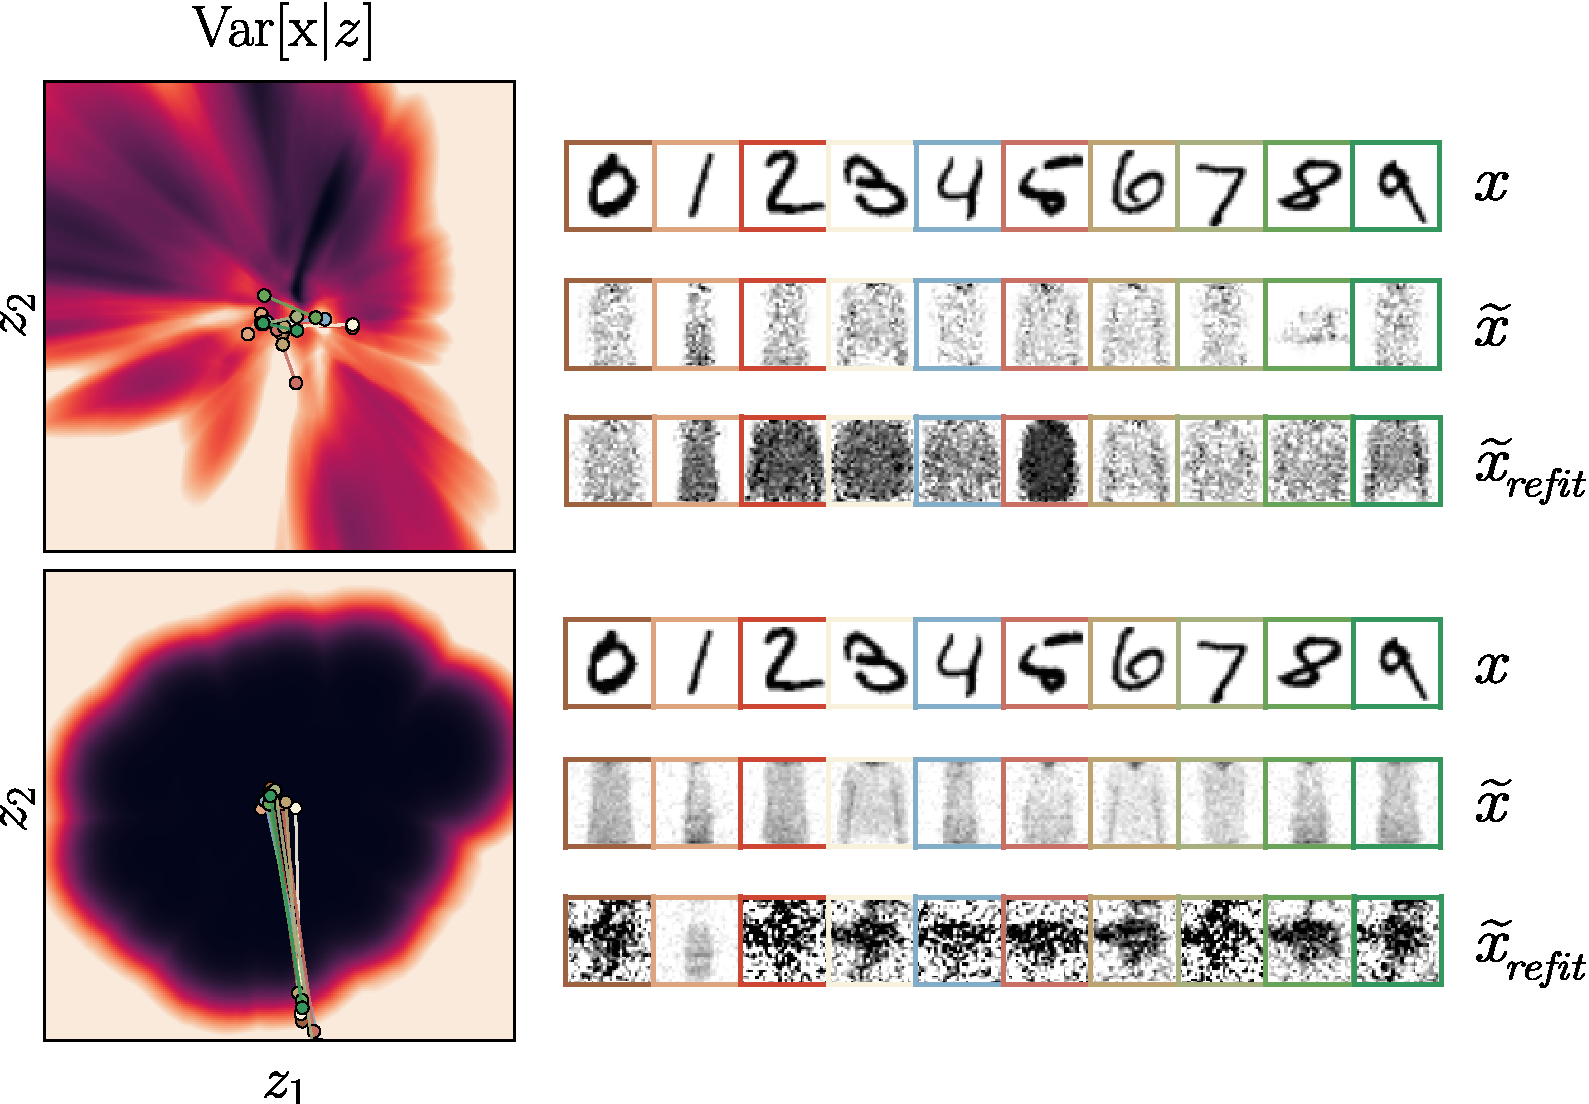
\includegraphics[width=\textwidth]{assets/re_encoding_plot.pdf} %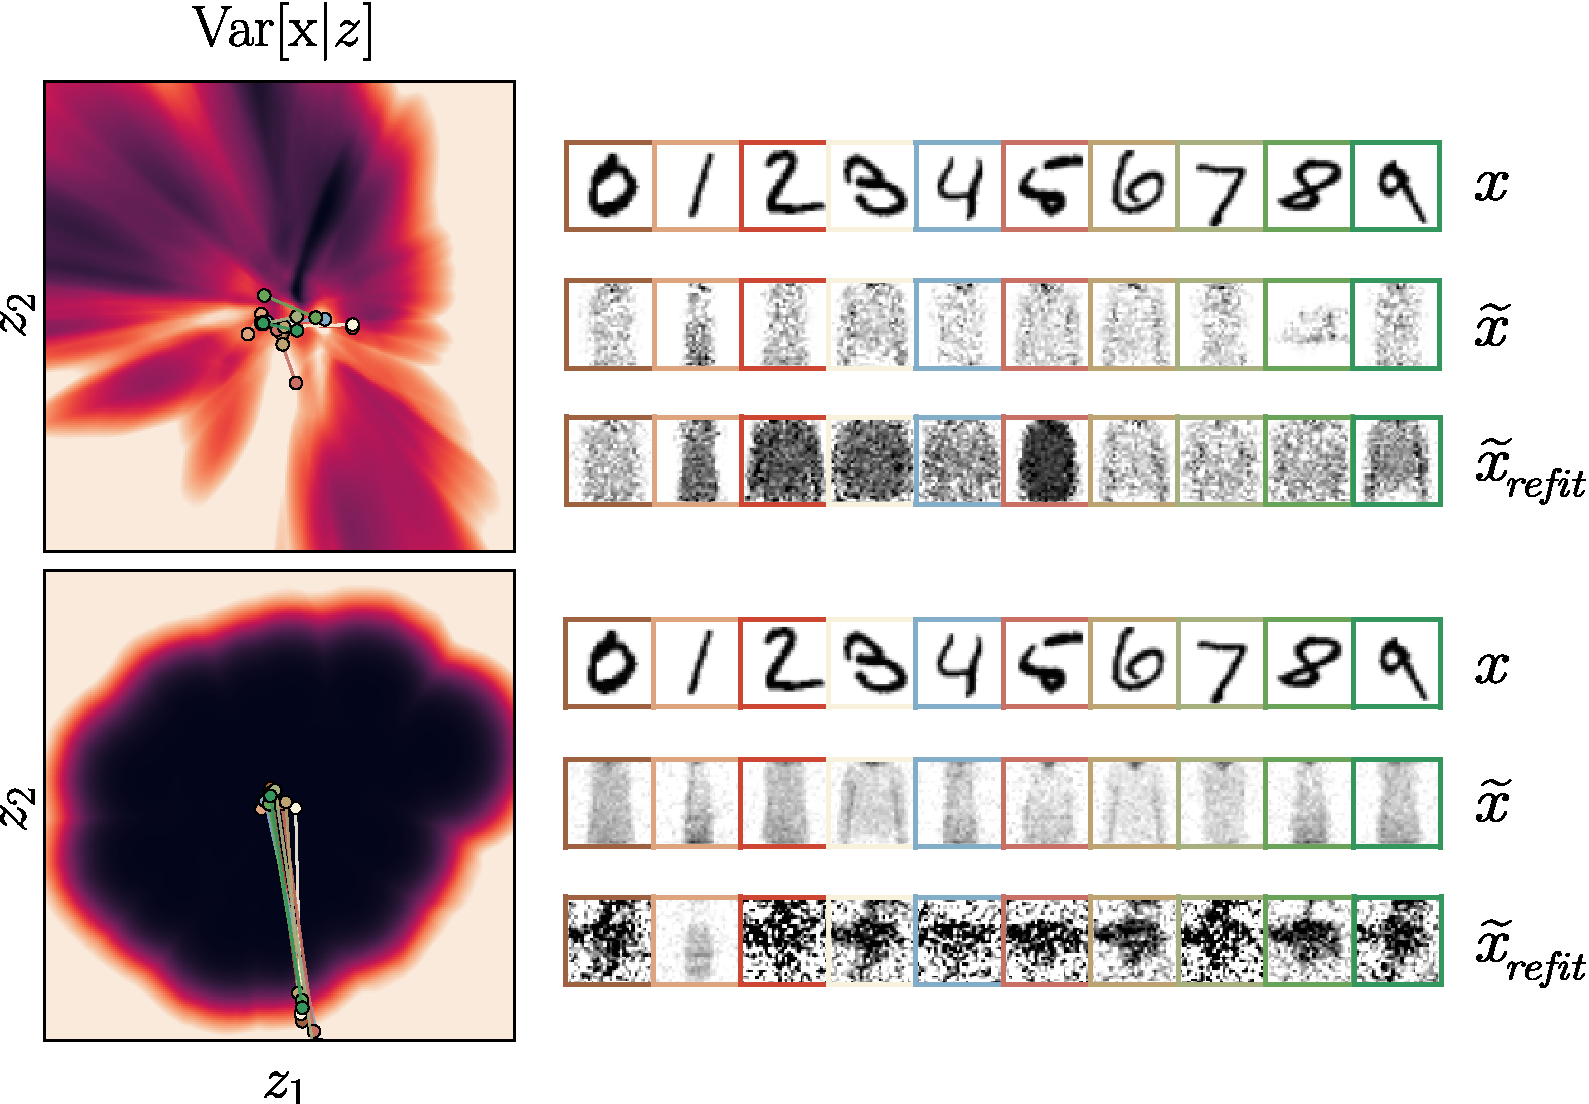
\includegraphics[height=5.05cm]{assets/re_encoding_plot.pdf}
      \vspace{-5.5mm}
      \captionof{figure}{Effect of encoder refitting on the latent representations (left) and corresponding samples (right). OOD inputs (first rows, $x$) initially result in in-distribution samples (second rows, $\tilde{x}$). The refitted encoder displaces the encodings (coloured trajectories), modifying the generated samples (third rows, $\tilde{x}_{\text{refit}}$).}
      \label{fig:re-encoding}
    \end{minipage}
    \hspace{.02\textwidth}
    \begin{minipage}[l]{.2\textwidth}
        \centering
        \vspace{-1.8cm}
        \includegraphics[width=4cm]{assets/show_vae_samples.pdf} % \includegraphics[height=5cm]{assets/vae_variance_plots.pdf}
        \vspace{-5.5mm}
        \captionof{figure}{Generated samples}
        \label{fig:show_vae_samples}
    \end{minipage}%
\end{figure*}

\clearpage

\onecolumn

\begin{table}[h]
\caption{UCI benchmarks - $\mathcal{L}$}
\label{tab:uci_benchmarks_elbo}
\input{../output/full-table-test_elbo↑}
\end{table}

\begin{table}[h]
\caption{UCI benchmarks - $\log p(y|x)$}
\label{tab:uci_benchmarks_log_p}  
\input{../output/full-table-test_expected_log_likelihood↑}
\end{table}

\clearpage

\begin{table}[h]
\caption{UCI benchmarks - $\text{RMSE}\left[y,\mu(x)\right]$}
\label{tab:uci_benchmarks_mean_rmse}
\input{../output/full-table-test_mean_fit_rmse↓}
\end{table}

\begin{table}[h]
\caption{UCI benchmarks - $\text{RMSE}\left[\Var[y|x],\left(y-\mu(x)\right)^2\right]$}
\label{tab:uci_benchmarks_variance_rmse}
\input{../output/full-table-test_variance_fit_rmse↓}
\end{table}

\begin{table}[ht]
\caption{UCI benchmarks - $\text{RMSE}\left[y,\tilde{y}\right]$}
\label{tab:uci_benchmarks_sample_rmse}
\input{../output/full-table-test_sample_fit_rmse↓}
\end{table}

\begin{table}[ht]
\caption{UCI benchmarks - $\mathbb{E}[\text{KL}]$}
\label{tab:uci_benchmarks_noiee_kl}
\input{../output/full-table-noise_kl_divergence↓}
\end{table}
  
\end{document}